\subsection{Filters}
A series of filters as recommended by the JetMET POG \cite{metFilters} are applied to
filter "bad" events, such as those where there is a huge difference in the \pt of
muon measured from the tracker and the muon chambers. Although the occurrence of such
"bad" events is rare, these filters are applied as sanity measures. These
filters mostly affect the actual data, most of them have no effect on the simulated
events. The efficiency of all combined filters is 99.4\% for data, and 99.9\%
for SM \ttjets MC sample. These filters are particularly useful in those
analyses where there is a requirement of very high missing transverse energy (MET)
and the final event yield is small. A detailed description of each filter is given
below:
\begin{itemize}
	\item \textbf{HBHE noise filter}: It is known that the barrel and endcap
		part of the HCAL records noise (sporadic anomalous signals) at a
		fixed
		rate even if there is no stable beam for physics data taking
        \cite{metFilters}. An event is supposed to have such a noise if the flag
		\verb|Flag_HBHENoiseFilter| is set to 1. Such an event is filtered.
	\item \textbf{HBHE isolated noise filter}: This filter first finds the
		candidates for rechits and rejects the event if the sum of
		iso-tagged energy is $>$ 50 GeV, the sum of iso-tagged transverse
		energy
		$>$ 25 GeV, and the number of iso-tagged rechits is $>$ 9. The flag
		\verb|Flag_HBHENoiseIsoFilter| is used for this purpose.
 	\item \textbf{CSC beam halo filter}: The actual physics objects of interest
		are those which are produced in the pp collision. However, there
		are machine induced particles, produced through beam-gas or
		beam-pipe interactions, which fly with the beam at a large radius
		(up to 5m). These machine induced particles are reconstructed mainly
		in the Cathode Strip Chambers (CSC) as muon candidate. A set of
		selection is applied through
        \verb|Flag_globalSuperTightHalo2016Filter| \cite{metFilters}. This flag is
		set to 1 if the CCS beam halo filter is applied and 0 if not applied.
	\item \textbf{Good primary vertex filter}: The events are required to have
		at least one good primary vertex. Therefore, those events are
		filtered where there is no good vertex. A good vertex is
		required to be real, the z-component of the position is $ <$ 24 cm,
		the $\rho$ component of the position $<$ 2 cm, and the minimum
		number of degrees of freedom are $>$ 4. The \verb|Flag_goodVertices|
		is set to 1 if the event has passed this filter.
	\item \textbf{Bad EE supercrystal filter}: The events are filtered if
		there is an unusually large energy deposit in the four superclusters
        of ECAL endcaps \cite{metFilters}. This filter is applied only on data
		through the \verb|Flag_eeBadScFilter|.
	\item \textbf{ECAL dead cell trigger primitive filter}: If the energy of
		the ECAL crystals are estimated from the trigger primitive and
		lies near the saturation energy then that event is filtered
        \cite{metFilters}. The \verb|Flag_EcalDeadCellTriggerPrimitiveFilter| flag
		is used to indicate if an event passes this filter or not.
	\item \textbf{Bad PF muon filter}: An event is filtered if the muon is
		although qualified as a PF muon but the quality is very low, and
		the \pt is large. The events are filtered if a muon is found
		which has \pt $>$ 100 GeV, segment compatibility $< 0.3$ or relative
		percentage error in the \pt of the best (inner) track is more than
		200\% (100\%), and $\Delta R$ (muon, PFmuon) $< 0.001$.
	\item \textbf{Bad charged hadron filter}: Those events are filtered where
		the quality of the muon is low and it is not declared as PF muon.
		However, this non-PF muon is used in the calculation of PF-MET
		as a candidate for charged hadron. To reject such events, the muon
		is required to have same \pt, segment compatibility, and error in
		track cuts as that of the above filter. An additional requirement
    of $\Delta R$ (muon, charge hadron) $<$ 0.00001, and \verb|PtDiffRell|
		$< 0.00001$ is applied where \verb|PtDiffRell| = (\pt of PF candidate - \pt
		of muon inner track)/(0.5* (\pt of PF candidate + \pt of muon inner
		track)).
\end{itemize}

All of the above filters are not directly stored in the trigger collection of the
\verb|MINIAOD| data set. The \verb|EDFilters| are used on the fly to apply unavailable
filters. The list of filters with their availability and pplicability is shown
in Table (\ref{tab:eventFilters}).
\begin{table}
\caption{ List of event filters applied to data and MC samples. Most of the filters
	are available in the {\em MINIAOD} through the trigger collection. The
	unavailable filters are applied on the fly using EDFilters.}
\label{tab:eventFilters}
\centering
\begin{adjustbox}{max width=\textwidth}
 \begin{tabular}{ccc}\hline\hline
  {\bf{Name of the filter}} & {\bf{Available in MINIAOD}} & {\bf{Applied on}}\\\hline\hline
  \verb|HBHE noise filter|            & Yes & Data \& MC \\
  \verb|HBHE isolated noise filter|   & Yes & Data \& MC \\
  \verb|CSC beam halo filter|         & Yes & Data \& MC \\
  \verb|Good primary vertex filter|   & Yes & Data \& MC \\
  \verb|Bad EE supercrystal filter|   & Yes & Data  \\
  \verb|ECAL dead cell trigger primitive filter| & Yes & Data \& MC\\
  \verb|Bad PF Muon Filter|  & No & Data \& MC \\
  \verb|Bad Charged Hadron Filter|        & No & Data \& MC \\\hline
 \end{tabular}
\end{adjustbox}
\end{table}


\subsection{Triggers}
The high-level triggers (HLT) are applied to select events enriched
with desired physics objects. The trigger conditions are stored in the form of
programming strings also called trigger paths. For every event, these paths are
stored. Depending on the topology of an analysis, an event is selected if the
corresponding trigger path is available in that event. For this analysis, an
event is selected if it has a trigger path of \verb|HLT_IsoMu24*| and
\verb|HLT_IsoTkMu24*| with logical \verb|OR| for the muon channel, and
\verb|HLT_Ele27_WPTight_Gsf| for electron channel. The efficiency of these
triggers depends on \pt and $\eta$ of the lepton. For lower Pt, the efficiency is
very poor and has a sudden increase at a particular value. That sudden increase is called trigger turn-on and the leptons are required to have \pt higher than that at the
turn-on.

The muon and electron trigger efficiency as a function of \pt is shown in Figure
(\ref{fig:trigEff}). The trigger turn-on for muon trigger is at about \pt = 24 GeV,
hence in the
subsequent selection, the muon is required to have \pt $>$ 26 GeV. For the electron
trigger (\verb|HLT_Ele27_WPTight_Gsf|), the trigger turn-on is a little higher at about
\pt = 33 GeV, therefore a cut of \pt $>$ 35 GeV is applied on electrons in the
subsequent selection.
\begin{figure}
     \centering
	\subfigure[Muon trigger efficiency \cite{ref:muon-twiki}]
     	{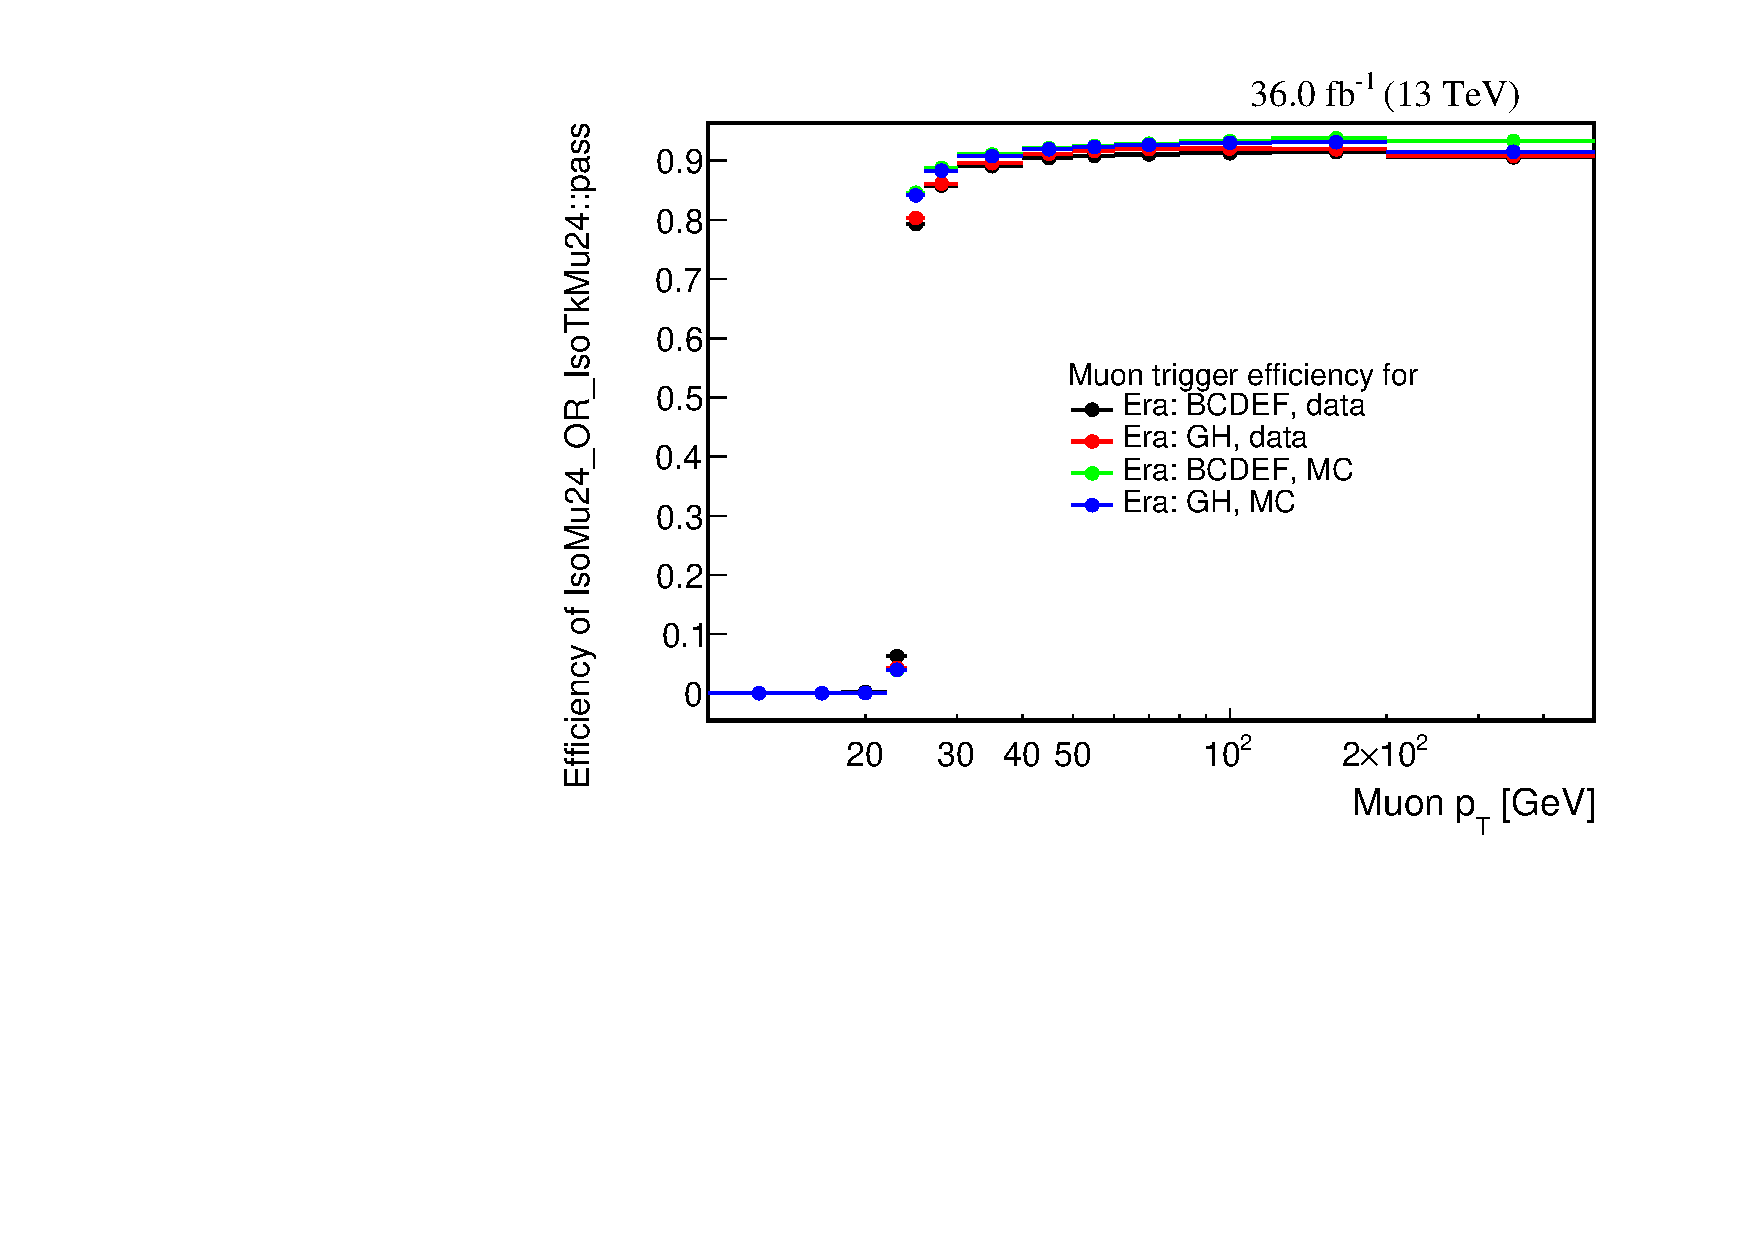
\includegraphics[width=0.60\linewidth]{Image/EffAndSF/muonTrigEff.pdf}}
     	\vfil
	\subfigure[Electron trigger efficiency in the barrel region \cite{eleTrigEff}]
     	{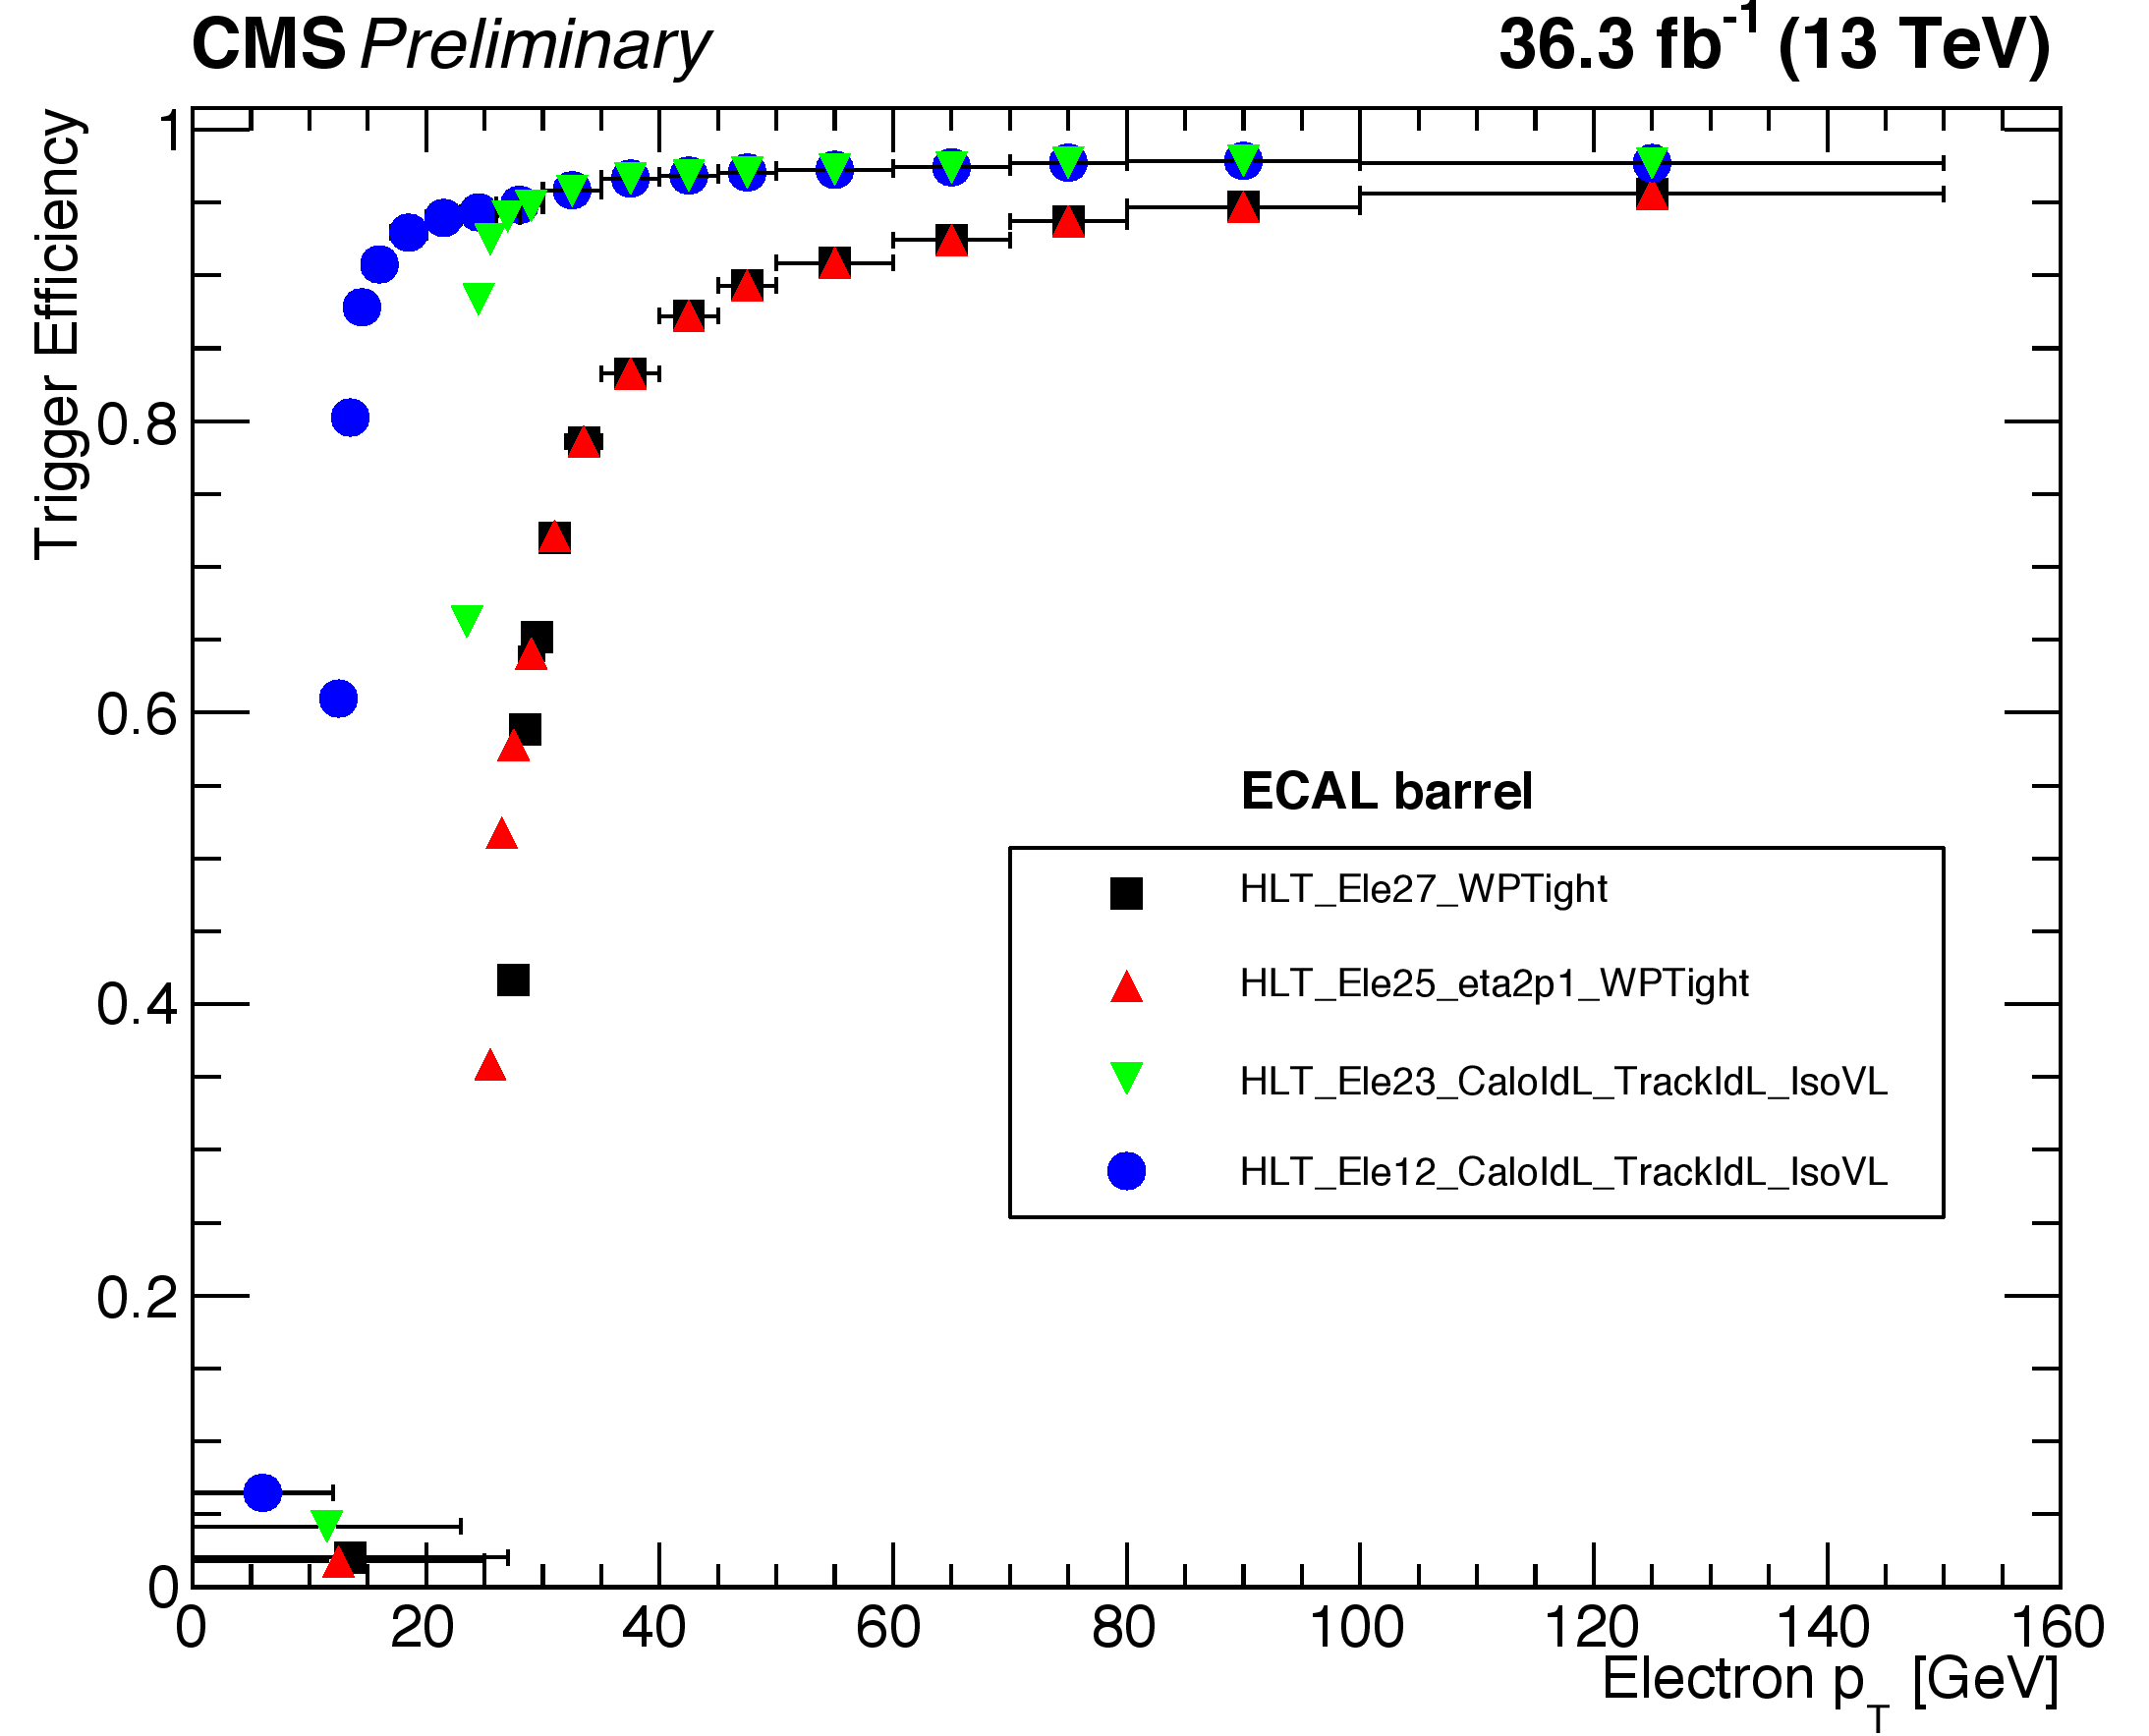
\includegraphics[width=0.49\linewidth]{Image/EffAndSF/eleTrigEB.png}}
	\subfigure[Electron trigger efficiency in the endcap region \cite{eleTrigEff}]
     	{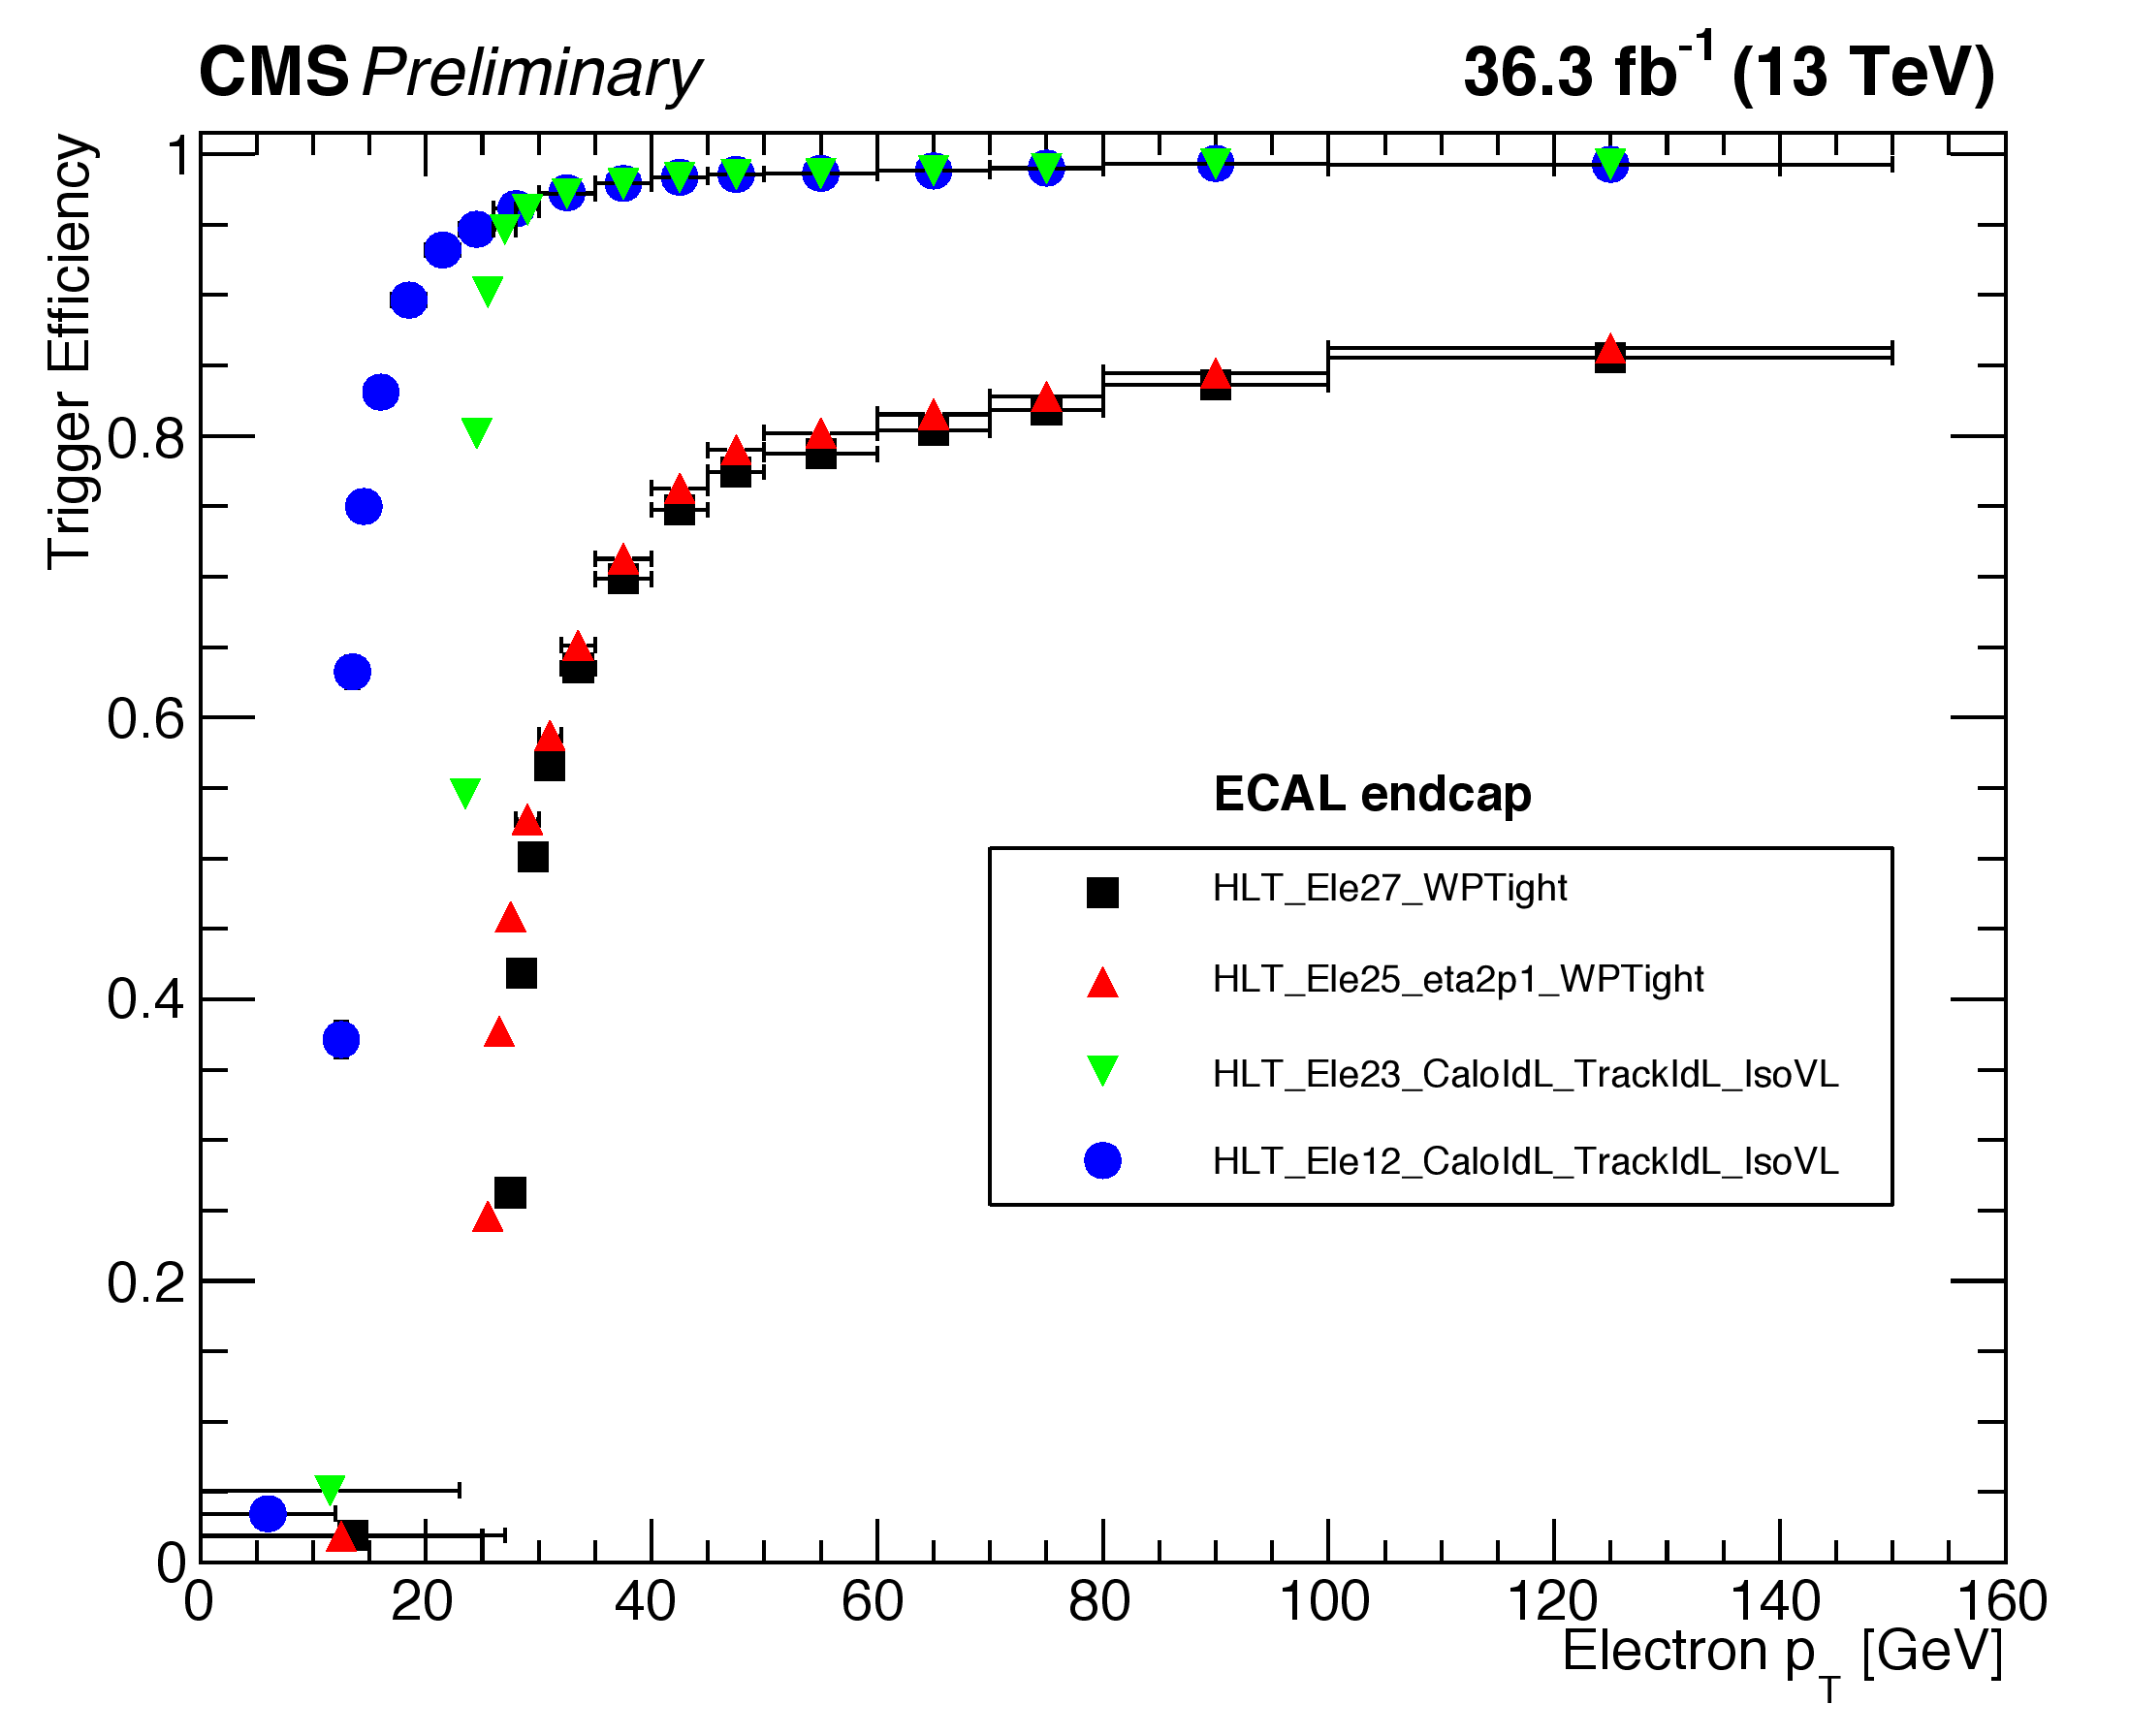
\includegraphics[width=0.49\linewidth]{Image/EffAndSF/eleTrigEE.png}}
	\caption{Muon and electron trigger efficiency as a function of transverse
	momentum. The trigger turn-on is at about \pt = 24 GeV for muon, and 33 GeV
	for electron (HLT\_Ele27\_WPTight\_Gsf) triggers.}
     \label{fig:trigEff}
 \end{figure}
